%%%CONTEMPORARY%%%
\documentclass[unnumsec,webpdf,contemporary,large]{oup-authoring-template}%

\graphicspath{{Fig/}}

% line numbers
%\usepackage[mathlines, switch]{lineno}
%\usepackage[right]{lineno}

\theoremstyle{thmstyleone}%
\newtheorem{theorem}{Theorem}%  meant for continuous numbers
%%\newtheorem{theorem}{Theorem}[section]% meant for sectionwise numbers
%% optional argument [theorem] produces theorem numbering sequence instead of independent numbers for Proposition
\newtheorem{proposition}[theorem]{Proposition}%
%%\newtheorem{proposition}{Proposition}% to get separate numbers for theorem and proposition etc.
\theoremstyle{thmstyletwo}%
\newtheorem{example}{Example}%
\newtheorem{remark}{Remark}%
\theoremstyle{thmstylethree}%
\newtheorem{definition}{Definition}

\begin{document}

% \journaltitle{Journal Title Here}
% \DOI{DOI HERE}
% \copyrightyear{2022}
% \pubyear{2019}
% \access{Advance Access Publication Date: Day Month Year}
% \appnotes{Paper}

% \firstpage{1}

%\subtitle{Subject Section}

\title[Short Article Title]{SNF-CNN: Predicting Comprehensive Drug-Drug Interaction via Similarity Network Fusion and Convolutional Neural Networks}
% [1,4,$\ast$]
% \author[1,3]{M.Amin Khodamoradi\ORCID{0000-0002-2700-5384}}
% \author[2]{ Bahareh Levian}
% \author[2]{Changiz Eslahchi}
% \author[3]{Maria Marques}
% \author[1,3]{Ricardo Jardim-Gonçalves}
% \author[4]{Fifth Author\ORCID{0000-0000-0000-0000}}

% \authormark{A. Khodamoradi et al.}

% \address[1]{\orgdiv{Universidade NOVA de Lisboa}, \orgname{NOVA School of Science and Technology (FCT NOVA)}, \orgaddress{\state{Caparica}, \country{Portugal}}}
% \address[2]{\orgdiv{Department of Computer Sciences}, \orgname{Shahid Beheshti University}, \orgaddress{\state{Tehran}, \country{Iran}}}

% \address[3]{
% \orgdiv{Center of Technology and Systems (UNINOVA-CTS) and Associated Lab of Intelligent Systems (LASI)}, \orgname{Organization}, \orgaddress{\state{Caparica}, \country{Portugal}}}

% \corresp[$\ast$]{Corresponding author. \href{email:Khodamoradi1992@gmail.com}{Khodamoradi1992@gmail.com}}

% \received{Date}{0}{Year}
% \revised{Date}{0}{Year}
% \accepted{Date}{0}{Year}
\abstract{This research addresses the critical need to identify drug-drug interactions (DDIs) before market entry. Existing preclinical detection methods are resource-intensive, prompting the use of computational models based on premarket drug properties. However, current models often oversimplify interactions, neglecting nuanced alterations in pharmacological effects. DDIs, rooted in the structural features of the DDI graph, are non-random, and understanding these relationships is vital for making comprehensive predictions and uncovering structural patterns in the DDI graph. The study introduces the Similarity Network Fusion and Convolutional Neural Networks (SNF-CNN) model, treating comprehensive DDIs as a signed network. SNF-CNN excels in predicting degressive (AUC = 0.975, AUPR = 0.967), enhancive (AUC = 0.969, AUPR = 0.822) DDIs, and Unknown DDIs (AUC = 0.971, AUPR = 0.948). Comparative analysis against state-of-the-art methods highlights SNF-CNN's superiority, not only in predicting DDIs but also in accurately forecasting non-DDIs. The SNF-CNN code and data are available on GitHub. For inquiries or collaboration, please contact \href{mailto: delbar.faghihmirzaei@kuleuven.be}{delbar.faghihmirzaei@kuleuven.be}.
% \textbf{Motivation}: Identifying drug-drug interactions (DDIs) before market entry is critical. While preclinical detection is resource-intensive, computational methods predict DDIs based on premarket drug properties. Existing models often focus on binary interactions, overlooking nuanced alterations in pharmacological effects. DDIs, rooted in the structural features of the DDI graph, are not random. Uncovering these relationships is crucial for understanding DDI mechanisms, guiding comprehensive predictions, and revealing structural patterns in the DDI graph for prescribing multiple drugs.\\
% Drug-drug interactions (DDIs) often lead to unexpected and adverse reactions, underscoring the critical need for their identification before market entry. However, preclinical detection of DDIs remains resource-intensive. Computational methods have demonstrated the ability to predict potential DDIs on a large scale using premarket drug properties. While many models focus on determining whether drugs interact, they frequently overlook the enhancive (positive) and degressive (negative) alterations of pharmacological effects. Furthermore, these complex DDIs are not random and may stem from the structural features of the DDI graph. Uncovering such relationships is essential for understanding the mechanisms behind DDI occurrences. Predicting comprehensive DDIs and elucidating structural patterns in the DDI graph provide crucial guidance for prescribing multiple drugs.\\
% \textbf{Results}: In this study, we treat a set of comprehensive DDIs as a signed network and introduce the Similarity Network Fusion and Convolutional Neural Networks (SNF-CNN) model for predicting the enhancive or depressive effects of drug pairs. SNF-CNN demonstrates strong performance in depressive DDI prediction (AUC = 0.975, AUPR = 0.967), enhancive DDI prediction (AUC = 0.969, AUPR = 0.822), and Unknown DDI prediction (AUC = 0.971, AUPR = 0.948). Comparative analysis against three state-of-the-art methods on our dataset highlights the superiority of SNF-CNN. This innovative approach excels not only in predicting comprehensive DDIs but also in accurately forecasting non-DDIs.\\
% \textbf{Availability and Implementation}: The code and data are available on the GitHub page of \href{https://github.com/aminkhod/DDI-Project}{SNF-CNN code and data} (\url{https://github.com/aminkhod/DDI-Project})\\
% \textbf{Contact}: \href{mailto: KA.khodamoradi@uninova.pt}{A.khodamoradi@uninova.pt}\\
% \textbf{Supplementary Information} Links to additional figures/data available on a website or reference to online-only supplementary data available at the journal's website.\\
% \begin{figure}[H]
%     \centering
%     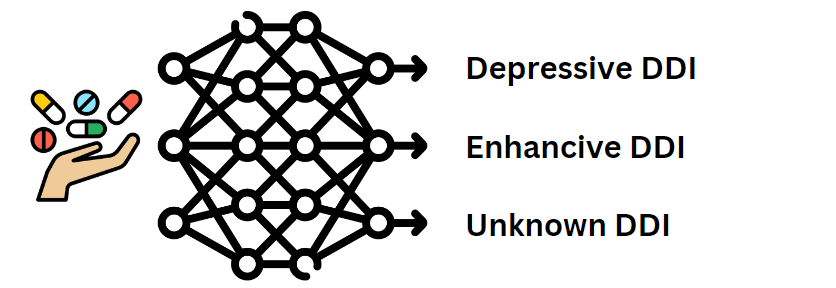
\includegraphics[scale=0.7]{doc/ddi.png}
%     % \caption{Graphical abstract}
%     \label{fig:GA}
% \end{figure}}
}
\keywords{Drug-Drug Interaction, Drug Similarity, Drug Similarity Integration, Feature Selection, Recommender System}

% \boxedtext{
% \begin{itemize}
% \item Key boxed text here.
% \item Key boxed text here.
% \item Key boxed text here.
% \end{itemize}}
\Abbreviations{DDI:Drug-drug interactions; CV:cross-validation; SNF:Similarity Network Fusion}

\maketitle


\section{Introduction}
When multiple drugs are taken together, their effects or behaviors may be unexpectedly influenced by each other~\cite{Wienkers2005}. This phenomenon is known as Drug-Drug Interaction (DDI), which can lead to reduced drug efficacy, increased toxicity, or other adverse reactions between the co-prescribed drugs. With the rising number of approved drugs, the incidence of unidentified DDIs is also increasing rapidly. For instance, among approved small molecular drugs listed in the Drug Bank, approximately 15 out of every 100 drug pairs have known DDIs~\cite{Law2014}. Such interactions pose risks to patients receiving multiple medications~\cite{Leape1995, PMID:28232141, Mulroy2017}. Understanding DDI is crucial as it is the first step in exploring drug combinations, which are increasingly seen as promising solutions for treating complex diseases~\cite{PMID:22219721}. Therefore, there is an urgent need for screening and analyzing DDIs before administering clinical co-medications. However, traditional DDI identification approaches, such as testing Cytochrome P450 or transporter-associated interactions, face challenges including high costs, lengthy duration, animal welfare concerns~\cite{Zhang2015}, limited trial participants, and a multitude of drug combinations undergoing screening in clinical trials. Consequently, only a few DDIs are identified during drug development, often in the clinical trial phase. Some are reported post-approval, while many are discovered during post-marketing surveillance~\cite{Karim2019}.

DDIs can be significantly influenced by a patient's medical history and genetics. To bridge these aspects, the Smart4Health project\footnote{\url{http://www.smart4health.eu}} developed two platforms: one personal, containing health information from the citizen (Citizen Health Data Platform – CHDP), including medical conditions, allergies, intolerances, medication use, and genetic data, and one de-identified, containing data donated for research by the citizen (Research Platform – RP). CHDP utilizes HL7 FHIR\footnote{\url{ https://hl7.org/fhir}} to structure collected data, while RP adopts OMOP CDM to convey data from CHDP and make it reusable by third-party research infrastructures (e.g., ELIXIR\footnote{\url{https://elixir-europe.org}}). The concept involves citizens collecting and aggregating data generated from interactions with medical institutions (e.g., medication prescriptions, laboratory results, discharge letters) into a single, interoperable EHR. This data may also encompass genetic data if available. This data can be donated to the RP at the citizens' discretion. Specifically regarding medication intake and genetic data, these are linked to drug exposure and outcome data within the OMOP CDM\footnote{\url{https://www.ohdsi.org/data-standardization}}. This mechanism has the potential to streamline data collection and contribute to ensuring data quality. Moreover, placing the citizen at the center of this process may expedite and broaden the identification of DDIs, facilitating a more comprehensive understanding of their mechanisms.

% Computational approaches are a promising alternative to discovering potential DDIs on a large scale, and they have recently gained attention from academia and industry~\cite{Barbara2016, Zhou2016}. Data mining-based computational approaches have been developed to detect DDIs from various sources~\cite{Zhang2015, Karim2019}, such as scientific literature~\cite{Bui2014, Zhang2016le} electronic medical records~\cite{Yamanishi2008}, and the Adverse Event Reporting System of the Food and Drug Administration (FDA\footnote{\url{http://www.fda.gov}}). Thus, these approaches rely on post-market clinical evidence. So, they cannot provide alerts of potential DDIs before clinical medications are administered. In contrast, machine learning-based computational approaches (e.g., Na\textcolor{red}{i}ve Similarity-Based Approach~\cite{Vilar2014}, Network Recommendation-Based~\cite{Zhang2015, Karim2019}, Classification-Based~\cite{Cheng2014}) can provide such alerts by utilizing pre-marketed or post-marketed drug attributes, such as drug features or similarities~\cite{Pahikkala2015}. These methods use different drug features to predict DDIs, such as chemical structures~\cite{Vilar2014}, targets~\cite{Luo2014}, hierarchical classification codes~\cite{Cheng2014}, side effects, and off-label side effects~\cite{Zhang2015, Karim2019, ShiHLLZY17}.
Computational approaches offer a promising avenue for discovering potential DDIs on a large scale, garnering recent attention from academia and industry~\cite{Barbara2016, Zhou2016}. Data mining-based computational methods have emerged to detect DDIs from diverse sources, including scientific literature~\cite{Bui2014, Zhang2016le}, electronic medical records~\cite{Yamanishi2008}, and the Food and Drug Administration's Adverse Event Reporting System (FDA\footnote{\url{http://www.fda.gov}}). However, these approaches rely on post-market clinical evidence, limiting their ability to provide alerts of potential DDIs before administering clinical medications. In contrast, machine learning-based computational methods (e.g., Naive Similarity-Based Approach~\cite{Vilar2014}, Network Recommendation-Based~\cite{Zhang2015, Karim2019}, Classification-Based~\cite{Cheng2014}) can offer such alerts by leveraging pre-marketed or post-marketed drug attributes, such as drug features or similarities~\cite{Pahikkala2015}. These approaches utilize various drug features to predict DDIs, including chemical structures~\cite{Vilar2014}, targets~\cite{Luo2014}, hierarchical classification codes~\cite{Cheng2014}, as well as side effects and off-label side effects~\cite{Zhang2015, Karim2019, ShiHLLZY17}.

% A dependency-based convolutional neural network (DCNN) was proposed by Liu et al. for drug-drug interaction extraction in 2016~\cite{shengyu2016}. DCNN is a text-mining approach that predicts DDIs based on unstructured biomedical literature and the existing knowledge bases. It applies convolution layers on word sequences and dependency parsing trees of candidate DDIs for adjacent words. DeepDDI has been proposed by~\cite{Ryu2018}, combining the structural similarity profile generation pipeline and Deep Neural Network (DNN). DeepDDI predicts DDIs from chemical structures and names of drug-drug or drug-food constituent pairs. It has various implications for adverse drug events, such as predicting potential causal mechanisms and using them for output sentences.
A dependency-based convolutional neural network (DCNN) was introduced by Liu et al. in 2016~\cite{shengyu2016} for extracting drug-drug interactions (DDIs). DCNN utilizes text-mining techniques to predict DDIs by analyzing unstructured biomedical literature and existing knowledge bases. It employs convolution layers to process word sequences and dependency parsing trees of potential DDIs for neighboring words. DeepDDI, developed by Ryu et al. in 2018~\cite{Ryu2018}, integrates a pipeline for generating structural similarity profiles with a Deep Neural Network (DNN). This approach predicts DDIs based on the chemical structures and names of drug-drug or drug-food constituent pairs. DeepDDI offers significant implications for identifying adverse drug events, including predicting potential causal mechanisms and generating informative output sentences.

% Although previous methods had great advances, more prediction accuracy is still needed. Exploiting more similarities may help to make more advances in this problem. Similarity Network Fusion (SNF)~\cite{Wang2014} is a competent method to integrate various similarities, which is used in numerous biological contexts~\cite{Olayan2018, Tian2017, Kim2016}. The neural network is a strongly developed approach that provides satisfactory solutions, especially for large datasets and nonlinear analyses~\cite{Wang2016}, widely used in critical problems~\cite{HUANG2009, Fu2017, Pan2016}.
% Most of these existing machine learning approaches are designed to predict the typical two-class problem, which only indicates how likely a pair of drugs is a DDI. However, two interacting drugs may change their pharmacological behaviors or effects (e.g., increasing or decreasing serum concentration) in vivo. For example, the serum concentration of Flunisolide (DrugBank Id: DB00180) decreases when it is taken with Mitotane (DrugBank Id: DB00648), whereas its serum concentration increases when taken with Roxithromycin (DrugBank Id: DB00778). The first case is degressive DDI, and the second is enhancive DDI, which contains drug changes regarding pharmacological effects. It is more important to know whether the interaction increases or decreases the drug’s pharmaceutical behaviors, especially when making optimal patient care, establishing drug dosage, designing prophylactic drug therapy, or finding resistance to therapy with a drug~\cite{jan1981}.
While previous methods have made significant advances, achieving greater prediction accuracy remains a priority. Leveraging additional similarities could potentially lead to further advancements in this area. Similarity Network Fusion (SNF)~\cite{Olayan2018, Tian2017, Kim2016}. Neural networks represent a well-established approach, offering effective solutions, particularly for large datasets and nonlinear analyses~\cite{Wang2016}. They are widely utilized in critical problems across various domains~\cite{HUANG2009, Fu2017, Pan2016}.

Most existing machine-learning approaches focus on predicting the typical two-class problem, indicating the likelihood of a drug pair being a DDI. However, in vivo, two interacting drugs may alter their pharmacological behaviors or effects (e.g., by increasing or decreasing serum concentration). For instance, Flunisolide (DrugBank Id: DB00180) exhibits decreased serum concentration when taken with Mitotane (DrugBank Id: DB00648), while its serum concentration increases when taken with Roxithromycin (DrugBank Id: DB00778). These scenarios represent degressive and enhancive DDIs, respectively, involving changes in pharmacological effects. Understanding whether an interaction enhances or diminishes a drug's pharmaceutical behaviors is crucial for optimal patient care, establishing drug dosage, designing prophylactic drug therapy, and identifying resistance to therapy with a drug~\cite{jan1981}.

% Although the occurrence of both enhancive and degressive DDIs is not random~\cite{Shi2018, Yu2018}, most current approaches have not yet exploited this structural property and have been developed only for conventional two-class DDIs. Furthermore, revealing such a structural relationship is very important because it can help to understand how the DDIs occur. It is one of the most important steps for treating complex diseases~\cite{Cokol2017} and guides physicians in preparing safer prescriptions for high-order drug interaction.
While the occurrence of both enhancive and degressive DDIs is not arbitrary~\cite{Shi2018, Yu2018}, many current approaches have not capitalized on this structural property. Instead, they have primarily focused on conventional two-class DDIs. However, uncovering such a structural relationship is crucial for understanding the mechanisms underlying DDIs. It represents a significant step in the treatment of complex diseases~\cite{Cokol2017} and aids physicians in crafting safer prescriptions, particularly for high-order drug interactions.

Recent research has focused on addressing two key issues: 1) predicting three-class DDIs instead of the traditional two-class prediction, and 2) extracting the topological information of drugs in a DDI network.

The TMFUF model, introduced by Shi et al. in 2018~\cite{Shi2018}, aims to predict enhancive and degressive DDIs for different scenarios involving new drugs with no known DDI history. On the other hand, the DDINMF model, proposed by Yu et al.~\cite{Yu2018}, not only predicts DDIs but also assigns each drug to a drug community. Consequently, correlations emerge between drug communities and the numbers of enhancive, degressive, sum, and difference of DDIs for each drug.

These observations suggest that enhancive or degressive DDIs are not random but rather exhibit certain topological features in the DDI network. The BRSNMF model, proposed by Shi et al. in 2019~\cite{Shi2019}, utilizes Semi-NMF to predict degressive and enhancive DDIs more accurately, particularly in cold start scenarios~\cite{lesly2018}. This method leverages the Drug Binding Protein (DBP) feature to map new drugs (those without any known DDIs) with known drugs (i.e., drugs that have at least one DDI). The results demonstrate that BRSNMF defines drug communities with more moderate sizes by incorporating a regularization term into the Semi-NMF objective function based on the weakly balanced theorem.

All three introduced algorithms employ matrix factorization methods, adopting a network recommender-based approach. The matrix factorization approach, with slight modifications, has garnered significant attention from researchers as a suitable solution for predicting DDIs. However, these methods do not address potential DDIs, which are essential for prescribing drugs safely.

In this study, we outline the data preparation process and introduce a recommendation system designed to identify pairs of non-interacting drugs accurately. Subsequently, we introduce a groundbreaking algorithm that integrates drug similarities and utilizes deep learning recommendation systems to predict Drug-Drug Interactions (DDIs) within a comprehensive three-class model. Named 'Predicting Comprehensive Drug-Drug Interaction via Similarity Network Fusion and Convolutional Neural Networks' (SNF-CNN), this algorithm aims to uncover unknown and potential DDIs that have not been previously detected. Leveraging off-label side effects and the chemical structure of drugs embedded in our approach provides valuable insights into uncovering hidden potential DDIs within the existing DDI network. We harness the power of Similarity Network Fusion (SNF) to utilize similarity features effectively.

This approach diverges from conventional methods by relying on deep neural networks, specifically a convolutional neural network, and markedly differs from matrix factorization techniques. While we acknowledge alternative methods briefly, it is crucial to emphasize that our work represents a unique exploration within the realm of three-class data, distinguishing it from existing studies.
\bibliographystyle{plain}
\bibliography{reference}
\end{document}